%Document Class
\documentclass{latex/emulateapj}
\usepackage{multirow,color,wrapfig,ulem}

%Packages and Commands
%PACKAGES
\usepackage{multirow,color,wrapfig,ulem}
\usepackage {graphicx}
\usepackage{graphics}
\usepackage[dvips]{epsfig}

%COMMANDS
\newcommand{\kms}{{\ifmmode{{\mathrm{\,km\ s}^{-1}}}\else{\,km~s$^{-1}$}\fi}}
\newcommand{\lya}{{Ly-$\alpha$~}}
\newcommand{\ang}{{$\theta_{gal}$~}}
\newcommand{\lognh}{{$\log{n_H}$~}}
\newcommand{\nh}{{$n_H$~}}
\newcommand{\vel}{{$v_{out}$~}}
\newcommand{\vgal}{{$v_{gal}$~}}
\newcommand{\vout}{{$v_{out}$~}}
\newcommand{\avg}[1]{\langle{#1}\rangle}
\newcommand{\nscatt}{\langle N_{\rm  scatt}\rangle}
\newcommand{\hMpc}{{\ifmmode{h^{-1}{\rm Mpc}}\else{$h^{-1}$Mpc }\fi}}
\newcommand{\hGpc}{{\ifmmode{h^{-1}{\rm Gpc}}\else{$h^{-1}$Gpc }\fi}}
\newcommand{\hmpc}{{\ifmmode{h^{-1}{\rm Mpc}}\else{$h^{-1}$Mpc }\fi}}
\newcommand{\hkpc}{{\ifmmode{h^{-1}{\rm kpc}}\else{$h^{-1}$kpc }\fi}}
\newcommand{\hMsun}{{\ifmmode{h^{-1}{\rm{M_{\odot}}}}\else{$h^{-1}{\rm{M_{\odot}}}$}\fi}}
\newcommand{\hmsun}{{\ifmmode{h^{-1}{\rm{M_{\odot}}}}\else{$h^{-1}{\rm{M_{\odot}}}$}\fi}}
\newcommand{\Msun}{{\ifmmode{{\rm {M_{\odot}}}}\else{${\rm{M_{\odot}}}$}\fi}}
\newcommand{\msun}{{\ifmmode{{\rm {M_{\odot}}}}\else{${\rm{M_{\odot}}}$}\fi}}
\newcommand{\clara}{{\texttt{CLARA}}~}
\newcommand{\rand}{{\ifmmode{{\mathcal{R}}}\else{${\mathcal{R}}$ }\fi}}
\newcommand{\hs}{{\hspace{1mm}}}

\begin{document}

\title{Influence of galaxy rotation and outflows in the Lyman-$\alpha$ spectral line}
\shorttitle{Influence of galaxy rotation and outflows in the Lyman-$\alpha$ spectral line}

\shortauthors{Remolina-Gutierrez et al.}

\author{Maria Camila Remolina-Gutierrez, Jaime E. Forero-Romero \& Juan N. Garavito-Camargo} 
\affil{Departamento de F\'{i}sica, Universidad de los Andes, Cra. 1 No. 18A-10, Edificio Ip, Bogot\'a, Colombia}
\email{mc.remolina197@uniandes.edu.co}
\email{je.forero@uniandes.edu.co}
\email{jn.garavito57@uniandes.edu.co}

\keywords{Galaxies: high-redshift, Lyman Alpha Emission, Galaxy Rotation, Galaxy Outflows, Radiative Transfer}  

\begin{abstract}
\noindent ------------------------------------------------------------------------------------------------------------------------------------\\
MISSING: The abstract\\
------------------------------------------------------------------------------------------------------------------------------------\\
\end{abstract}

\section{Introduction}
\label{sec:intro}

%1.1 Lyman alpha line
%1.2 Models
%1.3 Overview 

\subsection{The Lyman Alpha emission line}

The Lyman Alpha ( \lya) emission line is the spectral line produced by an excited hydrogen atom when its electron jumps from the second energy level to the first one. This fall causes an emission of a photon with a corresponding wavelenght of $1215.67$ $\AA$. The whole Lyman series was discovered in 1906 by the american physicist Theodore Lyman. \\

%(TESIS) se extiende como se descubrió, formula, etc

In 1967 \cite{PartridgePeebles} predicted that young galaxies would have a strong \lya  emission. Nowadays galaxies selected using the \lya line are known as Lyman Alpha Emitters (LAEs). Since the first observed LAE by \cite{DjorgovskiThompson} different teams have observed several LAEs \citep{Rhoads00,Gawiser2007,Koehler2007,Ouchi08,Yamada2012,Schenker2012,Kulas12, Yamada2012, Chonis2013,Finkelstein2013,Ostlin14,Hayes2014,Faisst2014, Fumagalli2015} specially at $z\geq2$ since it is when the  line is redshifted into the optical regime. LAEs became then a tool to explore the extragalactic Universe and with upcoming telescopes such as the James Webb Space Telescope, new ones are going to be discovered with a better resolution and at higher redshifts. This creates a clear motivation to model them and observe them. \\

As for motivation, these observations have a direct impact in studying the reionization epoch \cite{review}, properties of the interstellar medium (ISM) and the intergalactic medium (IGM) \citep{Behrens13} \citep{DijkstraKramer}, constraining star formation rates of high redshift galaxies, understanding galaxy luminosity functions \cite{Max} and studying the large scale structure of the Universe. In all of these studies, an understanding of the processes that model the morphology and radiate transfer process behind the \lya line, is required. To fully understand the observed spectra of the LAEs, these galaxies must be modeled. \\

\subsection{Existing models of Lyman Alpha Emitters}

The resonant nature of the \lya line makes modelling it a challenging task, but constraining the nature of LAEs using the line is a common and strong objective. Analytical solutions for the outcoming spectra in simple ISM static geometries have been derived \citep{Adams72, Harrington73, Neufeld90, Dijkstra06}. Radiative transfer codes \citep{DijkstraKramer, Laursen09, Verhamme06, CLARA} have been developed in order to understand the effect of the gas kinematics in the \lya line. Special attention have been devoted to  the effects of clumpy media \citep{Hansen06} and expanding/contracting shell/spherical geometries started to be studied \citep{Ahn03,Verhamme06,Dijkstra06}. Hydrodynamic simulations have studied the outcomming spectra of LAEs in large scale simulations \cite{Forero12}. Escape of \lya photons at the line center is also a proposed model that fits the observations in a more accurate way \citep{Martin2015, Garavito14, Neufeld91}. And Monte Carlo codes have been used in hydrodynamic simulations to study in detail individual galaxies \citep{Laursen09,Barnes11,Verhamme12,Yajima12}.\\

Special attention have been devoted to model the presence of outflows in these galaxies, motivated by previous observational studies. Outflows are a consequence of the interstellar medium (ISM) being ejected from the galaxy due to supernova explosions. Here different models have attempt to simulate more realistic situations involving shell models and cavities \citep{Behrens2014}. Blue wings and bumps have been modeled when the outflows regulating the escape of \lya photons are still engulfed within a static interstellar medium \citep{Chung2015}. \cite{Verhamme06} created an expanding shell model that despite its geometric simplicity, has been able to fit several \lya profiles including: observational, as the ones studied by \cite{Hashimoto2015} who reproduced the sources \lya lines and calculated their outflow velocities, and simulated, as the ones created by \cite{Gronke2015} who determined if degeneracies exist between the different shell model parameters. Also, \cite{Orsi12} creates a wind shell model that could be interpreted as an expanding sphere. \cite{Rivera-Thorsen2015} found that no one single effect dominates in governing \lya radiative transfer and escape, and that \lya peak velocities are consistent with a simple model of an intrinsic emission line overlaid by a blueshifted absorption profile from the outflowing wind.\\

Despite the fact that outflows have been broadly studied, rotation should also be present in these galaxies. Recently, a rotation model, created by Garavito et al. \cite{Garavito14} models a rotating spherical galaxy with homogeneous gas mixture and analyzes that impact in the \lya line. However not a lot of attention has been payed to this effect in LAEs.\\

The joint effect of the above properties should have a direct impact on the morphology of the \lya line. This is the subject of this work. \\

\subsection{Paper Overview}

We propose a simplified model in which the galaxy is modeled as an sphere undergoing solid-body rotation, with an homogeneous mixture of dust and hydrogen at a constant temperature, that is also expanding in the radial direction due to outflows. In this model the optical depth \tauh, the  rotation velocity \vrot and the outflow velocity \vout are free parameters. \\

This paper is structured as follows. In \S \ref{sec:theo} we explain in detail the model of rotation and outflow that we use. In \S \ref{sec:results} we present the results of our model, specially how the morphology of the line changes with the free parameters. In \S \ref{sec:discussion} we compare our results with a recent observation of a LAE. In the latest section \S \ref{sec:conclusions} we present our conclusions and possible future work. Finally, in the appendix, we present the results of a \lya modeled only with the rotation analytical soution by \cite{Garavito14} that then is filtered by a \cite{Verhamme06} expanding shell.\\

\section{Theoretical Background}
\label{sec:theo}
In this section we describe the proposed model used to reproduce a real and consistent \lya profile. \\ 

\subsection{Model}

We use the simplified rotation model developed by \citep{Garavito14} in which a rotating galaxy is modeled as a solid rotating sphere, with a homogeneous mixture of hydrogen and dust. There is also the radial expanding velocity. Photons are initially at the center of the sphere. These two velocities are added by components as follows. The equations governing this movement in which the axis of rotation is defined to be align with the $z$-axis are: \\

\begin{equation}
v_{x}=\frac{x}{R}v_{\rm out}-\frac{y}{R}v_{\rm rot}, \label{subeq1}
\end{equation}

\begin{equation}
v_{y}=\frac{y}{R}v_{\rm out}+\frac{x}{R}v_{\rm rot}, \label{subeq2}
\end{equation}

\begin{equation}
v_{z}=\frac{z}{R}v_{\rm out}, \label{subeq3}
\end{equation}

Where $R$ is the radius of the sphere. The minus/plus sign in the $x$/$y$-component of the rotation velocity part indicates the direction of rotation. In this case we take the angular velocity in the same direction as the $\hat{k}$ unit vector. \\

CAMBIAR ESTOOOOO\\ 

(...) At the end only a fraction of those manage to get out of the outflow and their wavelengths are measured to find the final spectrum. In order to simulate all the possible cases we set some key parameters for the program to vary, and some others fixed which are defined by the characteristics of LAEs. This are chosen as follows.\\

\subsection{Galaxy Parameters}

Our aim is to provide a realistic baseline to compare against observations of LAEs at $z\sim 3$. It has been found by analysis of the abundance and angular correlation function that LAEs reside in DM halos of masses in the range $10^{10}-10^{11}$\Msun \cite{WalkerSoler2012}. This mass range corresponds to maximum circular velocities in the range $60-125$\kms and a median halo scale radius of $15$kpc. \footnote{These results were found using the  N-body data available in \url{www.cosmosim.org}}. \\

CAMBIAR ESTOOOOO (cambie 10E9 por 10E10)\\

These galaxies have gas fractions close to $20\%$ \citep{Narayanan2012}. We approximate that the hydrogen content is $20\%$ the total baryonic content from the cosmological baryon to dark matter  abundances $\Omega_b/\Omega_{dm}=0.1825$ \citep{Planck2015}, multiplied by a primordial Hydrogen fraction of $0.75$. All these considerations gives us hydrogen masses in the range $2.7\times 10^{8}-2.7\times 10^{9}$\Msun.\\

These choices give us a range for the number density of Hydrogen atoms of $4\times10^{-4}-4\times 10^{-3}$ atoms cm$^{-3}$. With a Lyman-$\alpha$ cross section at the line center of $\sigma_{H}=1.0\times 10^{-14}$ cm$^{2}$ we finally obtain that the optical depth from the cloud's center  should be in the range $\tau_{\rm H}=2 \times 10^{5} - 2 \times 10^{6}$.  \\

In order to be able to tell the influence of the rotation and outflow velocities in the \lya line morphology, a mapping of them is made without concerning of their physical meaning at first. The following ranges are selected for these parameters: \vrot in $0,100,200,300$ \kms and \vout in $100,200,300$ \kms.\\

%From these constraints we chose to model two kinds of central galaxies in the extremes of these distributions. The first has $\tau =2\times 10^5$ and a rotational velocity of $60$\kms. The second has $\tau=2\times 10^6$ and a rotational velocity of $125$\kms.\\

%For the first stage there are two fixed parameters: the optical depth $\tau = 10^8$ and the galaxy viewing angle \ang = $90^\circ$. For the second stage there is one fixed parameter: the metallicity of the outflow $Z=-4.0$. This 3 fixed values are selected because the characteristics of observed LAEs, especially their low mass and their highest star formation rate of all. \\

%We have then 3 parameters left that are going to vary along a wide range. These are: the galaxy rotation velocity \vrot, the outflow hydrogen column density \nh and the outflow expanding velocity \vout.\\ 

%\vrot covers 3 different angles: $20$ \kms, $100$ \kms and $200$ \kms. \lognh takes 41 different values from $20.0$ to $22.5$. And \vout covers 5 equidistant velocities from $100$ \kms to $500$ \kms. The permutations of these three are analyzed in section \ref{sec:results}. \\

%The results of this project consist of emulating a LAE spectrum basing on its physical characteristics defined by the 3 free parameters we stated before. When defined the combination of those three. \\

%In the following subsection each free parameter is explained deeper. \\

%In order to study the influence of each of the three free parameters, we fix two of them and see how the final spectrum varies along the other one left. In each case we will state these changes. \\

\section{Results}
\label{sec:results}

\begin{figure}[h!]
\begin{center}
  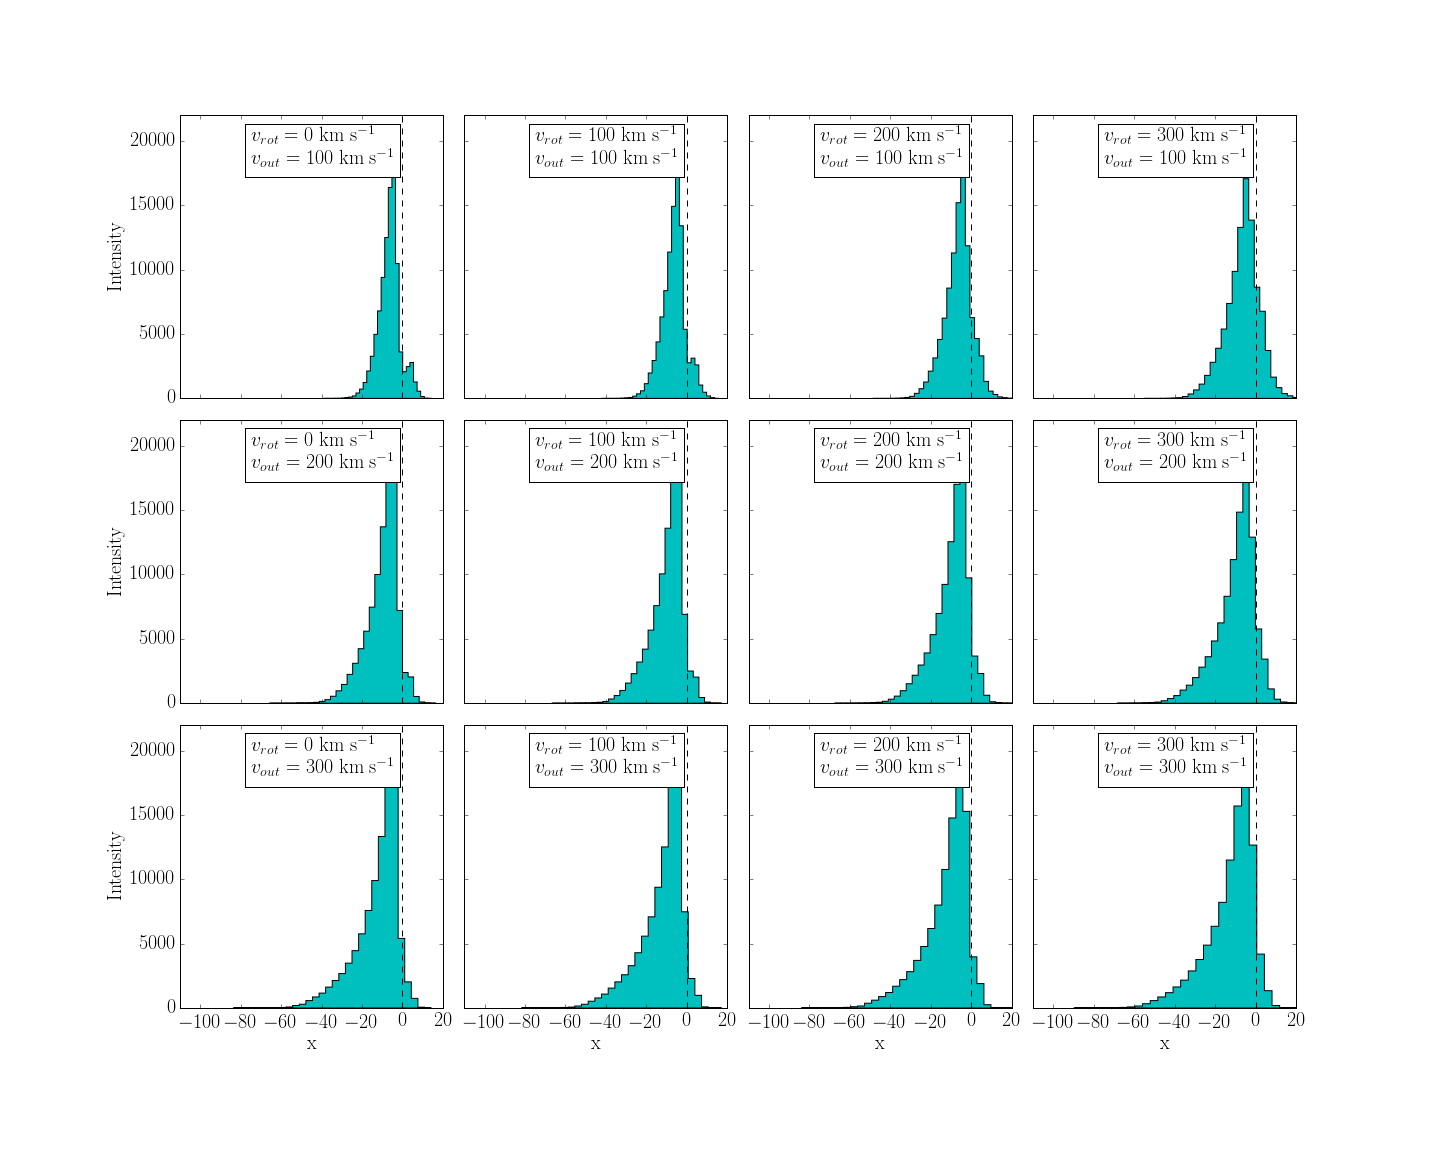
\includegraphics[width=0.5\textwidth]{./figures/tau10E5.png}
\end{center}
\caption{\textbf{\lya profile for \tauh$=10^5$:} With \vrot ranging $0,100,200,300$ \kms and \vout ranging $100,200,300$ \kms.
\label{fig:tau10E5}}
\end{figure}

\begin{figure}[h!]
\begin{center}
  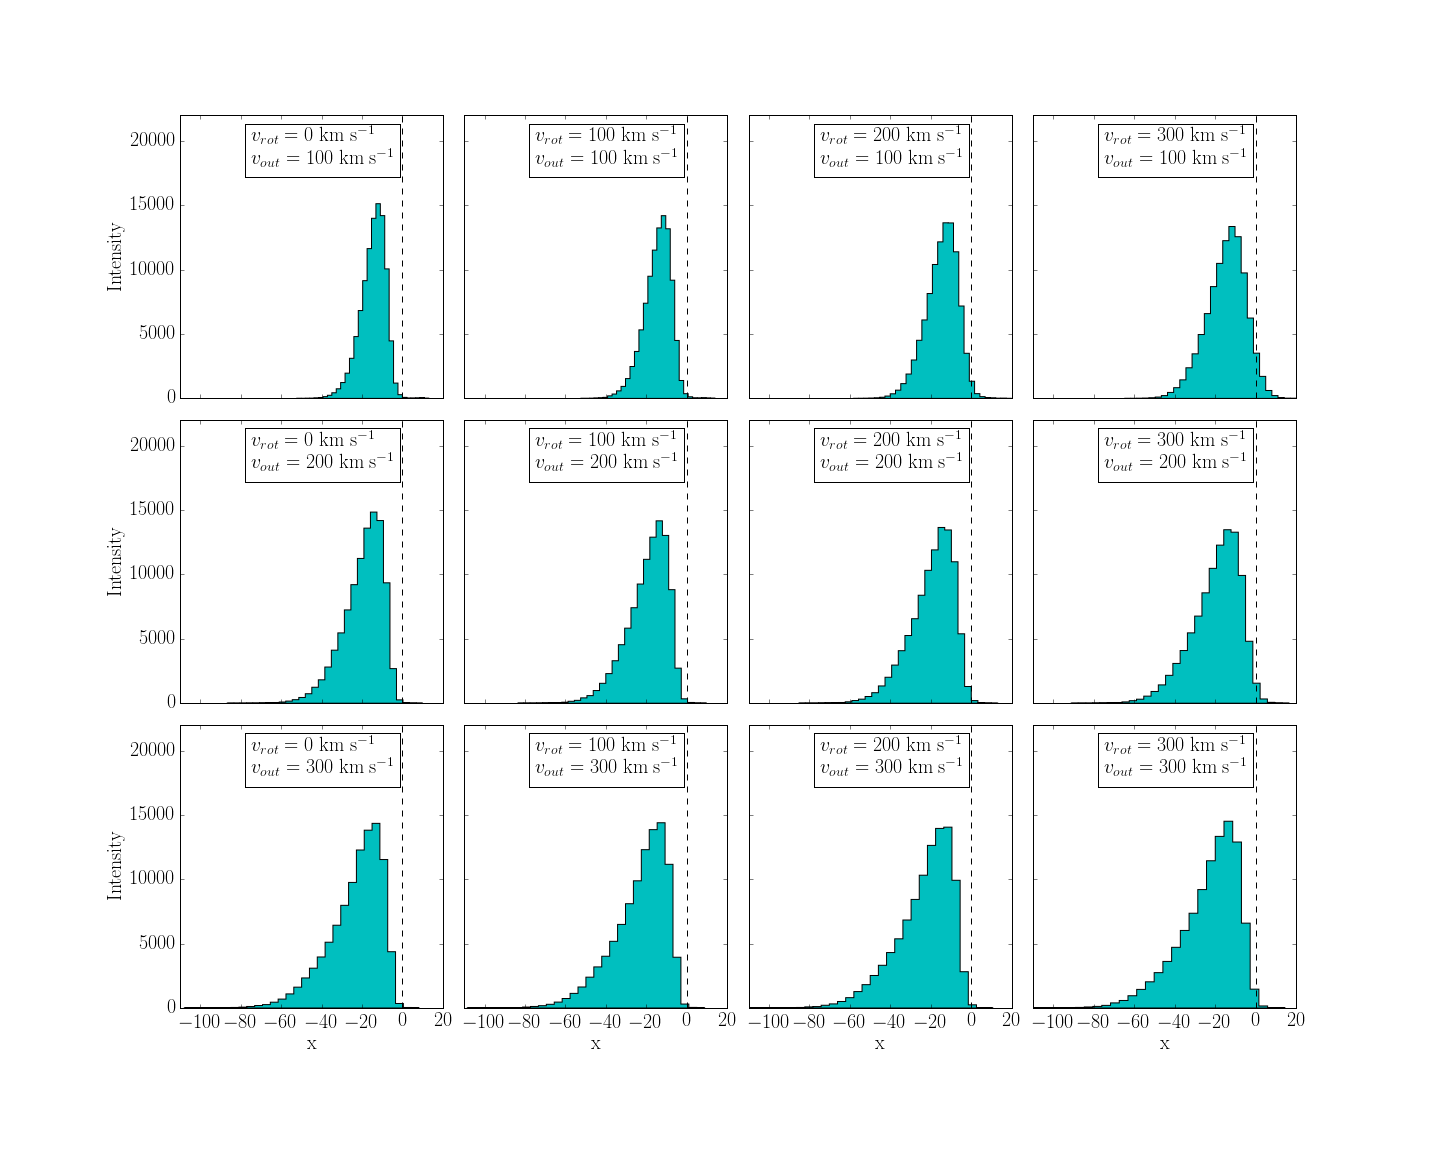
\includegraphics[width=0.5\textwidth]{./figures/tau10E6.png}
\end{center}
\caption{\textbf{\lya profile for \tauh$=10^6$:} With \vrot ranging $0,100,200,300$ \kms and \vout ranging $100,200,300$ \kms.
\label{fig:tau10E6}}
\end{figure}

\begin{figure}[h!]
\begin{center}
  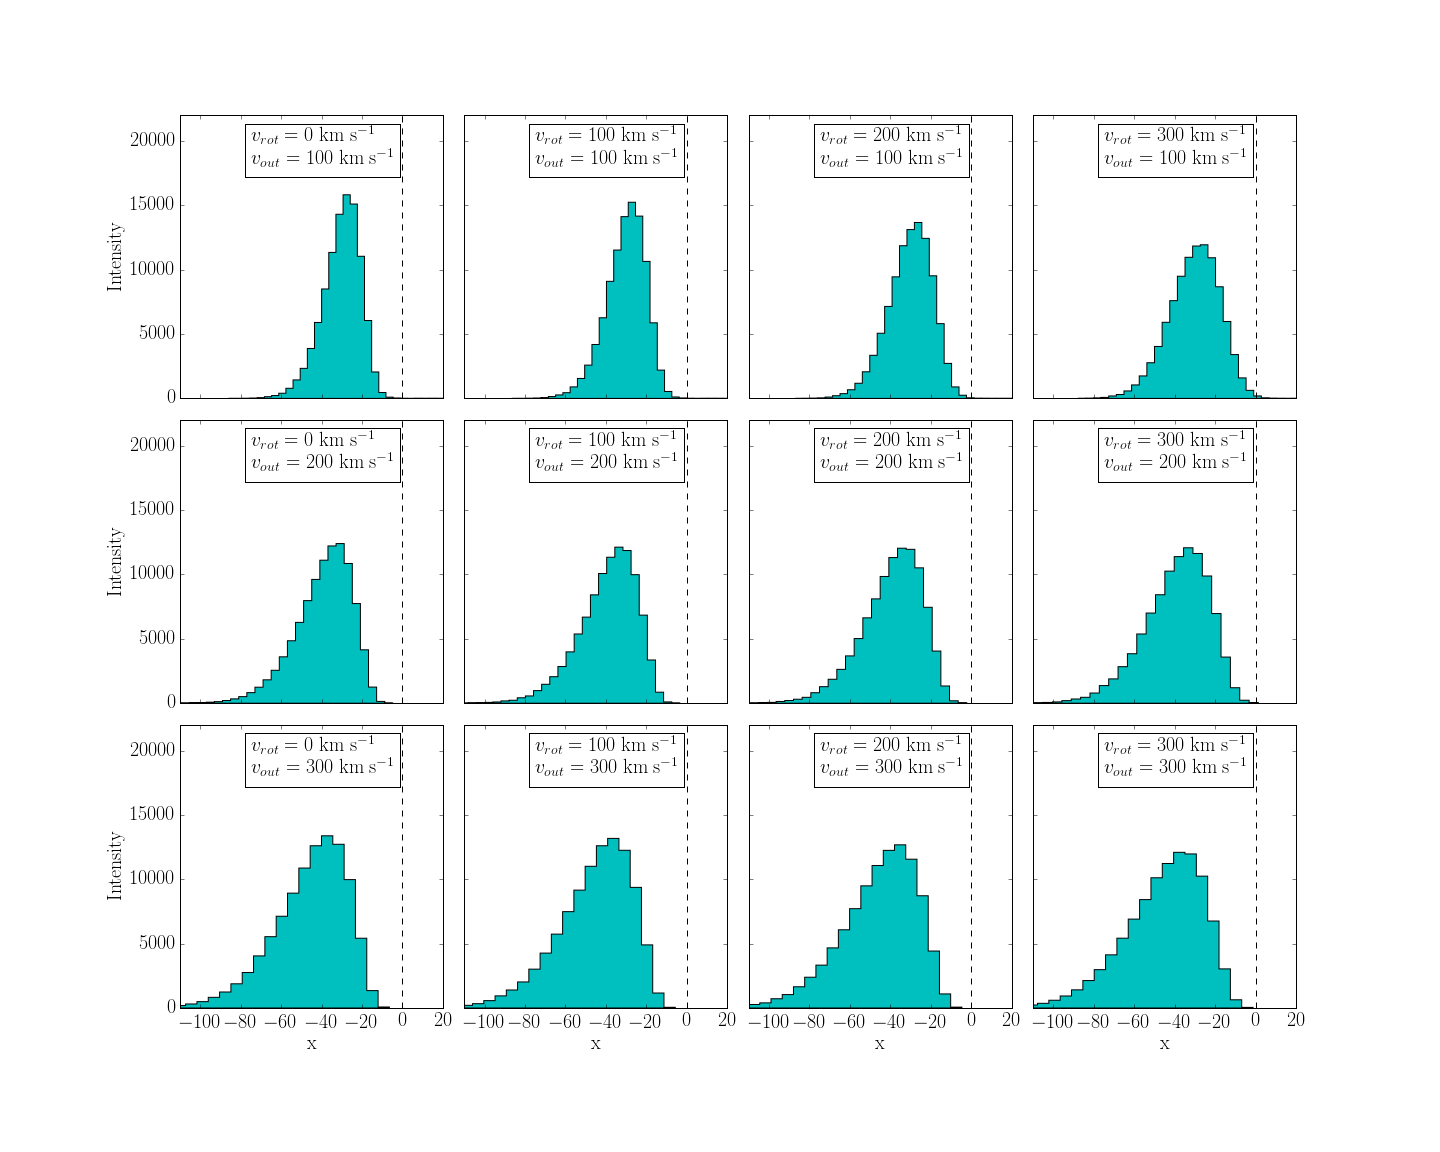
\includegraphics[width=0.5\textwidth]{./figures/tau10E7.png}
\end{center}
\caption{\textbf{\lya profile for \tauh$=10^7$:} With \vrot ranging $0,100,200,300$ \kms and \vout ranging $100,200,300$ \kms.
\label{fig:tau10E7}}
\end{figure}

\subsection{Influence of the Galaxy Rotation Velocity: \vrot}


\subsection{Influence of the Galaxy Outflow Velocity: \vout}


\subsection{Influence of the Galaxy Optical Depth: \tauh}


\subsection{Number of Peaks and Peaks Assymetry}


\section{Discussion}
\label{sec:discussion}

---------------------------------------------------------------------\\
TO ADD: \\
- Comparison with some other result (probably observations).\\
- Why is this result useful? \\
- What possible implications can this model have?\\
-----------------------------------------------------------------------\\

\section{Conclusions}
\label{sec:conclusions}
Here goes the conclusions....

\section*{Acknowledgments}

We acknowledge Alvaro Orsi and Julian Mejia for collaborating with us offering their time, advice and especially data. We used their outflow simulations in order to get our results in the appendix.\\

The data, source code and instructions to replicate the results of this paper can be found here {\texttt{https://github.com/mariacamilaremolinagutierrez/ LymanAlpha/}}.
Most of our code benefits from the work of the IPython and Matplotlib communities \citep{IPython,matplotlib}.\\

---------------------------------------------------------------------\\
MISSING: \\
- More acknowledgments.\\
-----------------------------------------------------------------------\\

%------------------------REFERENCES----------------------------

\bibliographystyle{latex/apj}
\bibliography{references}

\newpage

%------------------------APPENDIX----------------------------

\appendix
\section{Thin Shell Outflow}

In this section we describe the two different models that together are used to reproduce a real and consistent \lya profile. The first one is a rotation model for the galaxy and the second is a thin shell model for the outflow. \\ 

\subsection{Rotation Model}

We use the simplified rotation model developed by \citep{Garavito14} in which a rotating galaxy is modeled as a solid rotating sphere, with a homogeneous mixture of hydrogen and dust. Photons can be initially at the center or can be homogeneously distributed inside the sphere. The equations governing this solid-body rotation sphere in
which the axis of rotation is defined to be align with the $z$-axis are: \\

\begin{equation}
v_{x}=-\frac{y}{R}V_{\rm max}, \label{subeq1}
\end{equation}

\begin{equation}
v_{y}=\frac{x}{R}V_{\rm max}, \label{subeq2}
\end{equation}

\begin{equation}
v_{z}=0, \label{subeq3}
\end{equation}

Where $R$ is the radius of the sphere and $V_{\rm max}$ is the linear velocity at the sphere's surface. The minus/plus sign in the $x$/$y$-component of the velocity indicates the direction of rotation. In this case we take the angular velocity in the same direction as the $\hat{k}$ unit vector.\\

In this work we use the analytical expression for rotation derived in \citep{Garavito14} where a rotating sphere can be seen as a static sphere in the laboratory frame with a bulk velocity difference in each surface element with respect to a distant observer. With the previous analysis the outcoming spectra can be expressed as:\\

\begin{equation}
J(x,i) \approx 2\pi \int_0^Rdb \hs b
\int_0^{2\pi}d\phi \hs J(x,b,\phi,i),
\end{equation}

Where $J(x, b, \phi, i)$ is the spectrum of the flux emerging from the surface at point $(b, \phi)$ and is expressed as: 

\begin{equation}
J(x,b,\phi,i)=\frac{\sqrt{\pi}}{\sqrt{24}a\tau_0}\Bigg{(}\frac{(x-x_{\rm
    b})^2}{1+{\rm cosh}\Big{[}\sqrt{\frac{2\pi^3}{27}}\frac{|(x-x_{\rm
        b})^3|}{a\tau_0}\Big{]}}\Bigg{)} 
\end{equation}


\subsection{Outflow Model: Thin Shell}

We use an outflow model that follows the characteristics put described in \citep{Verhamme06} with the code presented in\citep{Orsi12}.  The outflow consists of an isothermal, spherical flow expanding at
constant velocity \vout.  The outflow is empty inside the shell's inner radius $R_{in}$ and reaches out to an external radius $R_{out}$. The relationship between these two radii is parameterized by $R_{in} =
f_{th}R_{out}$, with $f_{th}=0.9$ as the fiducial value. The temperature of the medium is assumed constant and equal to $T=10^4 K$ which sets the velocity dispersion of Maxwell-Boltzmann distributions to $v_{\rm th}=12.84$\kms. \\

The gas has an homogeneous Hydrogen number density inside the flow. The total mass inside the shell is parameterized by its column density\\

\begin{equation}
\label{eq:nh}
N_H = \frac{X_H M_{shell}}{4\pi m_H {R^2}_{out}},
\end{equation}
%
where $M_{shell}$ is the outflow mass, $m_H$ is the mass of the hydrogen atom and $X_H=0.74$ is the fraction of hydrogen in the cold gas.\\

The outflow also includes dust homogeneously mixed with the gas. The dust optical depth $\tau_d$ is parameterized by the metallicity of the cold gas $\langle Z_{cold} \rangle$: 

\begin{equation}
\label{eq:z}
\tau_{d} ???? \langle Z_{cold} \rangle
\end{equation}

\subsection{Joint Model}

The joint model consists of combining the two models that were just explained. A rotating spherical galaxy is placed at the center with a thin shell outflow surrounding it as seen in Fig. \ref{fig:model}. What happens is that the photons that escaped the galaxy enter now into the outflow with the same radial direction that they came out with. At the end only a fraction of those manage to get out of the outflow and their wavelengths are measured to find the final spectrum. \\

\begin{figure}[h!]
\begin{center}
  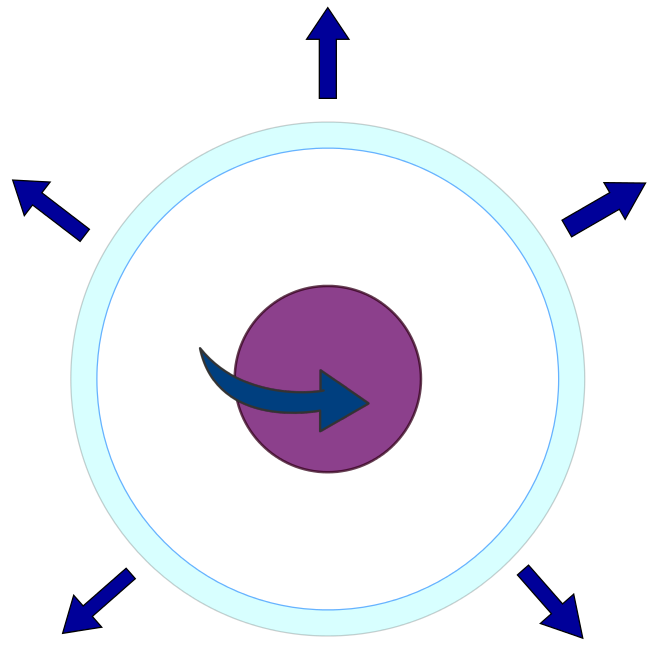
\includegraphics[width=0.3\textwidth]{./figures/model.png}
\end{center}
\caption{\textbf{Model:} A central rotating galaxy surrounded by an expanding thin shell outflow.
\label{fig:model}}
\end{figure}

In order to simulate all the possible cases we set some key parameters for the program to vary, and some others fixed which are defined by the characteristics of LAEs. This are chosen as follows.\\

\subsubsection{Galaxy Parameters}

Our aim is to provide a realistic baseline to compare against observations of LAES at $z\sim 3$. It has been found by analysis of the abundance and angular correlation function that LAES reside in DM halos of masses in the range $10^{10}-10^{11}$\Msun \cite{WalkerSoler2012}. This mass range corresponds to maximum circular velocities in the range $60-125$\kms and a median halo scale radius of $15$kpc.  \footnote{These results were found using the  N-body data available in \url{www.cosmosim.org}}. \\

These galaxies have gas fractions close to $20\%$ \citep{Narayanan2012}. We approximate that the hydrogen content is
$20\%$ the total baryonic content from the cosmological baryon to dark matter  abundances $\Omega_b/\Omega_{dm}=0.1825$ \citep{Planck2015}, multiplied by a primordial Hydrogen fraction of $0.75$.
All these considerations gives us hydrogen masses in the range $2.7\times 10^{8}-2.7\times 10^{9}$\Msun. \\

These choices give us a range for the number density of Hydrogen atoms of $4\times10^{-4}-4\times 10^{-3}$ atoms cm$^{-3}$. With a Lyman-$\alpha$ cross section at the line center of $\sigma_{H}=1.0\times 10^{-14}$ cm$^{2}$ we finally obtain that the optical depth from the cloud's center  should be in the range $\tau=2 \times 10^{5} - 2 \times 10^{6}$. \\

From these constraints we chose to model two kinds of central galaxies in the extremes of these distributions. The first has $\tau =2\times 10^5$ and a raotational velocity of $60$\kms. The second has $\tau=2\times 10^6$ and a rotational velocity of $125$\kms.\\

For the first stage there are two fixed parameters: the optical depth $\tau = 10^8$ and the galaxy viewing angle \ang = $90^\circ$. For the second stage there is one fixed parameter: the metallicity of the outflow $Z=-4.0$. This 3 fixed values are selected because the characteristics of observed LAEs, especially their low mass and their
highest star formation rate of all. \\

We have then 3 parameters left that are going to vary along a wide range. These are: the galaxy rotation velocity \vrot, the outflow hydrogen column density \nh and the outflow expanding velocity \vout. \\

\vrot covers 3 different angles: $20$ \kms, $100$ \kms and $200$ \kms. \lognh takes 41 different values from $20.0$ to $22.5$. And \vout covers 5 equidistant velocities from $100$ \kms to $500$ \kms. The permutations of these three are analyzed in section \ref{sec:results}. \\ 

The results of this project consist of emulating a LAE spectrum basing on its physical characteristics defined by the 3 free parameters we stated before. When defined the combination of those three. \\

In the following subsection each free parameter is explained deeper. \\

In order to study the influence of each of the three free parameters, we fix two of them and see how the final spectrum varies along the other one left. In each case we will state these changes.\\

\subsection{Influence of the Galaxy Rotation Velocity: \vrot}

If one sets fixed outflow \vout and \lognh in each case the rotation velocity has the same effect: it increases proportionally the intensities. However this change is not that significant. The resulting spectra are completely the same, but enlarged vertically by a small factor. Fig. \ref{fig:influence_vrot} helps visualize this effect in a better way.\\

\begin{figure}[h!]
\begin{center}
	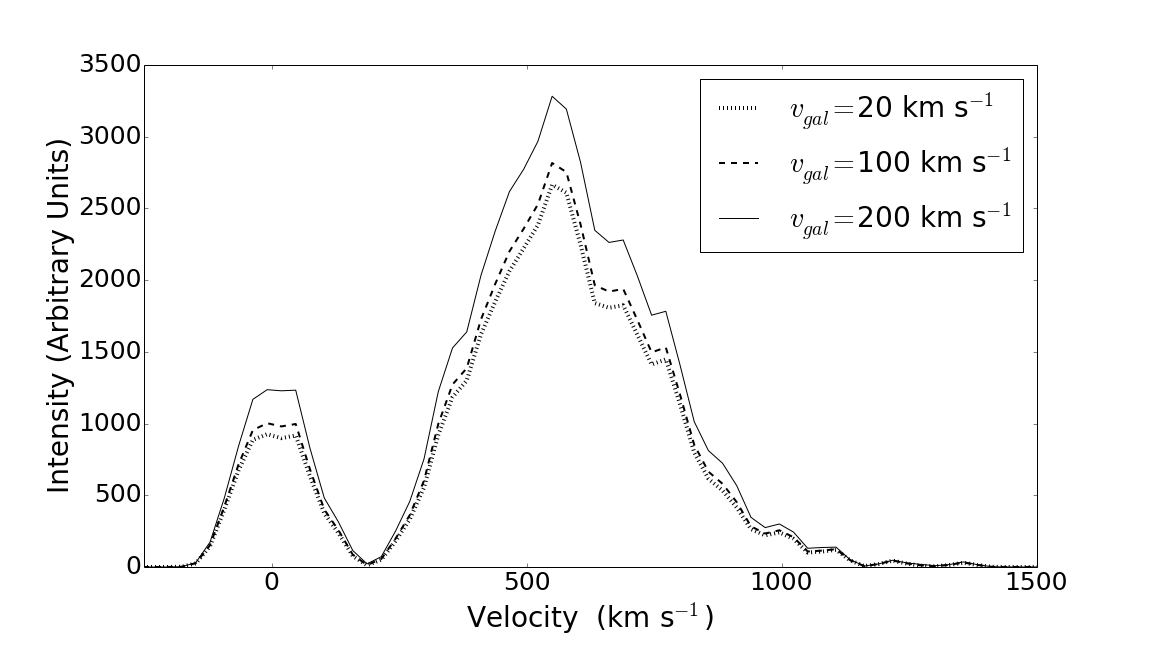
\includegraphics[width=0.5\textwidth]{./figures/inf_vgal_soft.png}
\end{center}
\caption{\textbf{Influence of Galaxy Rotation Velocity:} The values of the fixed parameters are \vout = $100$ \kms and \lognh = $20.9375$. The 3 possible velocities are shown in the plot with different line styles. The increase is visible as well as its small enlargement factor.\\
\label{fig:influence_vrot}}
\end{figure}

\subsection{Influence of the Outflow Hydrogen Column Density: \lognh }

The effect of the \lognh is the creation of 2 peaks: the left one very thin, tall and pronounced, and the right one very wide, small and soften. When the \lognh is increased, the left peak starts to decrease while mixing with the right one, decreasing their height ratio until the left peak completely disappears. The resulting spectrum, with high column density, is a wide single mountain with intensity significantly less than at the beginning. Fig. \ref{fig:influence_lognH} helps visualize this effect in a better way.\\

\begin{figure}[h!]
\begin{center}
  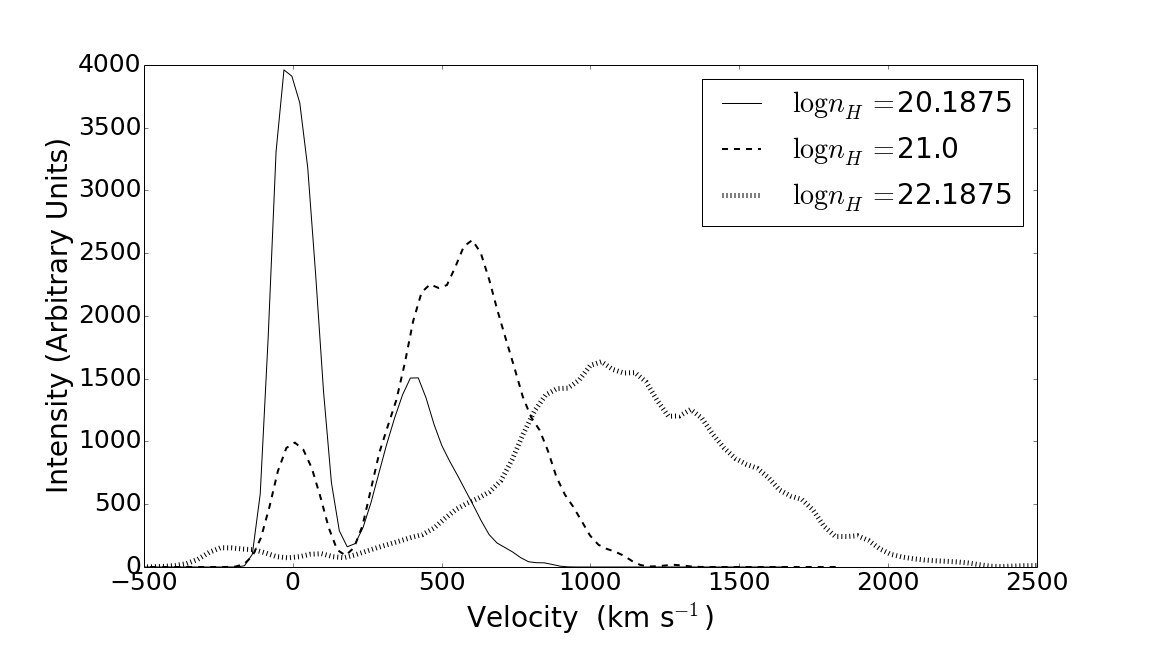
\includegraphics[width=0.5\textwidth]{./figures/inf_lognh_soft.png}
\end{center}
\caption{\textbf{Influence of Outflow Hydrogen Column Density:} The values of the fixed parameters are \vout = $100$ \kms and \vrot = $100$ \kms. There are three stages of the \lognh value shown: initial, intermediate and final, with the values shown on the plot.\\
\label{fig:influence_lognH}}
\end{figure}

\subsection{Influence of the Outflow Expanding Velocity: \vout }

The effect of this parameter consists in a shift of the initial spectrum in the column density. The more \vout the outflow has, the more the spectrum simulates the previous velocity but with a greater \lognh. If one compares with Fig. \ref{fig:influence_lognH} the similarities are really clear. \\

\begin{figure}[h!]
\begin{center}
  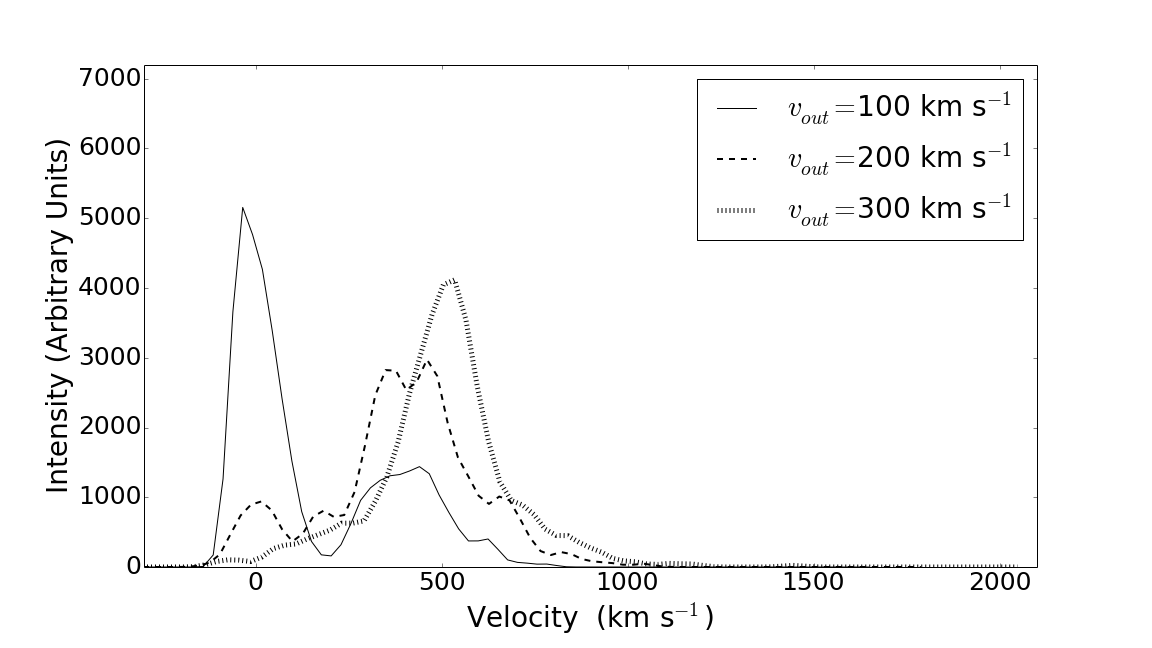
\includegraphics[width=0.5\textwidth]{./figures/inf_vout1_soft.png}
\end{center}
\caption{\textbf{Influence of Outflow Expanding Velocity:} The values of the fixed parameters are \lognh = 20.125 and \vrot = $100$ \kms.\\
\label{fig:influence_vout1}}
\end{figure}

\begin{figure}[h!]
\begin{center}
  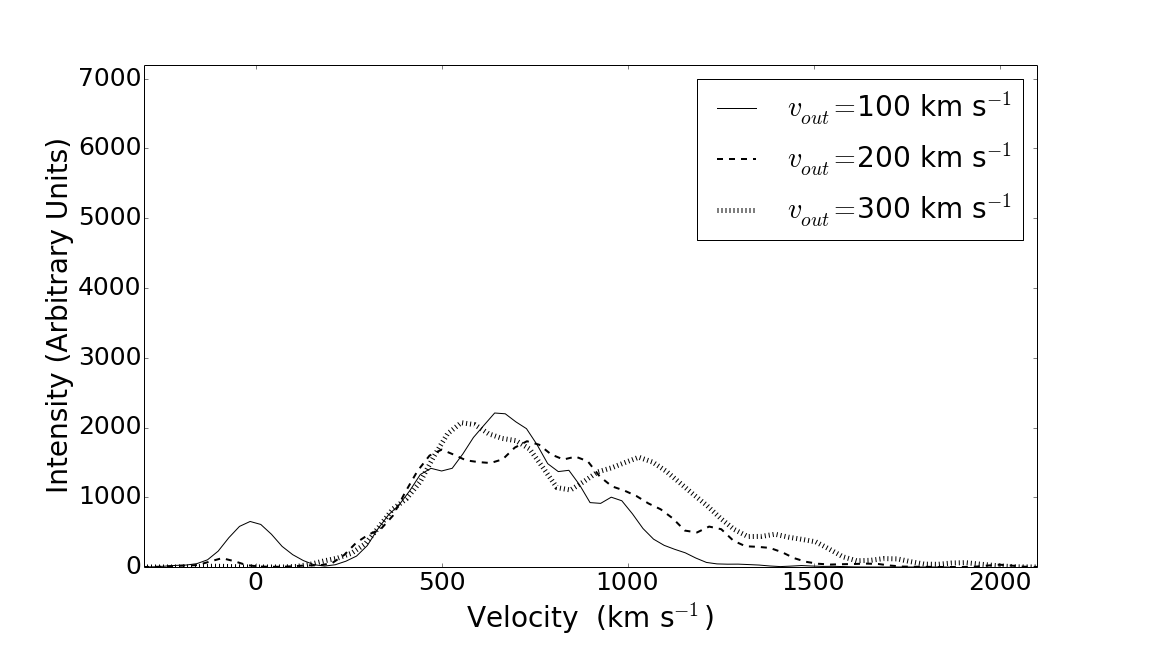
\includegraphics[width=0.5\textwidth]{./figures/inf_vout2_soft.png}
\end{center}
\caption{\textbf{Influence of Outflow Expanding Velocity:} The values of the fixed parameters are \lognh = 21.25 and \vrot = $100$ \kms.\\
\label{fig:influence_vout2}}
\end{figure}


%\section{Ejemplos para tener en cuenta}
%
%Ejemplo display math
%
%\begin{displaymath}
%J(x,b,\phi,i)=\frac{\sqrt{\pi}}{\sqrt{24}a\tau_0}\Bigg{(}\frac{(x-x_{\rm
%    b})^2}{1+{\rm cosh}\Big{[}\sqrt{\frac{2\pi^3}{27}}\frac{|(x
%      -x_{\rm b})^3|}{a\tau_0}\Big{]}}\Bigg{)},
%\end{displaymath}
%
%Ejemplo tabla
%
%\begin{table}
%\begin{center}
%\begin{tabular}{c cccccc}
%\hline \hline
%Source & $\tau_{H}$ & &  $\ V_{\rm max}$& & \\
%Distribution& &    & (\kms) & & \\
%& & 0 & 100 &200 & 300\\ \hline
%Homogeneous & $10^{5}$& 0.263 &  0.263 &  0.263 &  0.263  \\
%            & $10^{6}$ & 0.291 &   0.292 &  0.293 &  0.293 \\
%Central & $10^{5}$ &  0.096 & 0.096 &  0.096 & 0.096 \\
%  		&$10^{6}$ & 0.066 &  0.066 &  0.066 &  0.066 \\
%\hline
%\end{tabular}
%\caption{
% Ejemplo de tabla. }
%\label{table:escape}
%\end{center}
%\end{table}

\end{document}
